\chapter{Prezentacja warstwy użytkowej}
\label{chap:warstwa-uzytkowa}

\section{Ogólny układ interfejsu}

Warstwa użytkowa aplikacji \textit{IdentityCore} została przygotowana jako lokalny interfejs desktopowy utrzymany w ciemnym motywie. Po zalogowaniu większość widoków korzysta z tego samego układu: po lewej stronie znajduje się pionowe menu nawigacyjne z nazwą aplikacji, a po prawej główny obszar roboczy danego modułu. Aktualnie wybrany moduł jest wyróżniony innym tłem oraz akcentem kolorystycznym, dzięki czemu operator od razu widzi, w której części systemu aktualnie pracuje.

Wspólne menu boczne umożliwia przejście do panelu głównego, rejestru osób, identyfikacji twarzy, identyfikacji odcisku palca, historii prób oraz ustawień. W górnej części obszaru roboczego znajduje się tytuł widoku, krótki opis funkcji modułu oraz przycisk \texttt{Wyloguj}. Taki układ porządkuje sposób korzystania z aplikacji: operator najpierw wybiera moduł z menu, następnie pracuje w jego głównym panelu, a wyniki lub komunikaty są prezentowane w wydzielonych sekcjach widoku.

\section{Ekran logowania}

Pierwszym ekranem aplikacji jest ekran logowania. Jego zadaniem jest ograniczenie dostępu do głównej części systemu tylko do operatora posiadającego dane dostępowe. Po lewej stronie ekranu pokazano nazwę aplikacji, jej ogólne przeznaczenie oraz zakres dostępnych modułów. Po prawej stronie znajduje się formularz logowania z polami \texttt{Login} i \texttt{Hasło} oraz przyciskiem \texttt{Zaloguj}. Widoczna jest również informacja o koncie testowym, która ułatwia uruchomienie aplikacji w środowisku demonstracyjnym.
\begin{figure}[H]
    \centering
    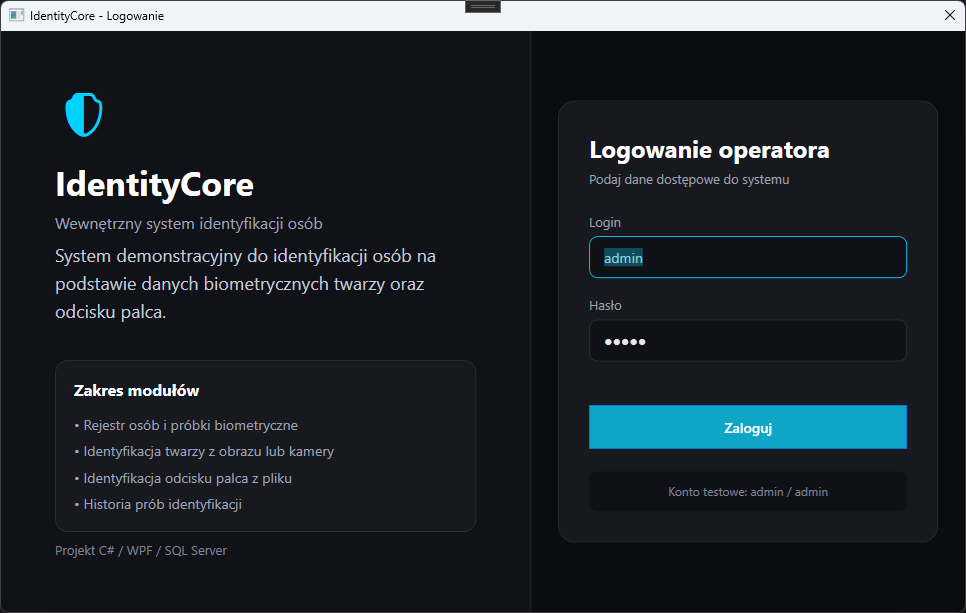
\includegraphics[width=0.98\textwidth]{figures/ui/ui_01_login.png}
    \caption{Ekran logowania do aplikacji IdentityCore}
    \label{fig:ui-login}
\end{figure}

\newpage

\section{Panel główny aplikacji}

Po poprawnym zalogowaniu operator trafia do panelu głównego. Jest to ekran podsumowujący aktualny stan systemu oraz najważniejsze dane zapisane w aplikacji. W górnej części panelu znajdują się kafle informujące o liczbie osób w bazie, liczbie osób z danymi biometrycznymi, liczbie szablonów twarzy, liczbie szablonów odcisków oraz liczbie zapisanych prób identyfikacji. Dzięki temu operator od razu widzi, czy system posiada dane potrzebne do wykonywania identyfikacji.

\bigskip

Centralna część panelu głównego prezentuje ostatnie próby identyfikacji. W tabeli widoczna jest data i czas próby, typ biometrii, dopasowanie, wynik oraz decyzja systemu. Prawa część widoku pokazuje gotowość danych biometrycznych, aktualne parametry rozpoznawania oraz szybkie przejścia do najważniejszych funkcji. Z tego miejsca operator może szybko przejść do rejestru osób, identyfikacji twarzy, identyfikacji odcisku lub historii prób, bez konieczności ręcznego wyszukiwania odpowiedniej funkcji w systemie.

\bigskip

\begin{figure}[H]
    \centering
    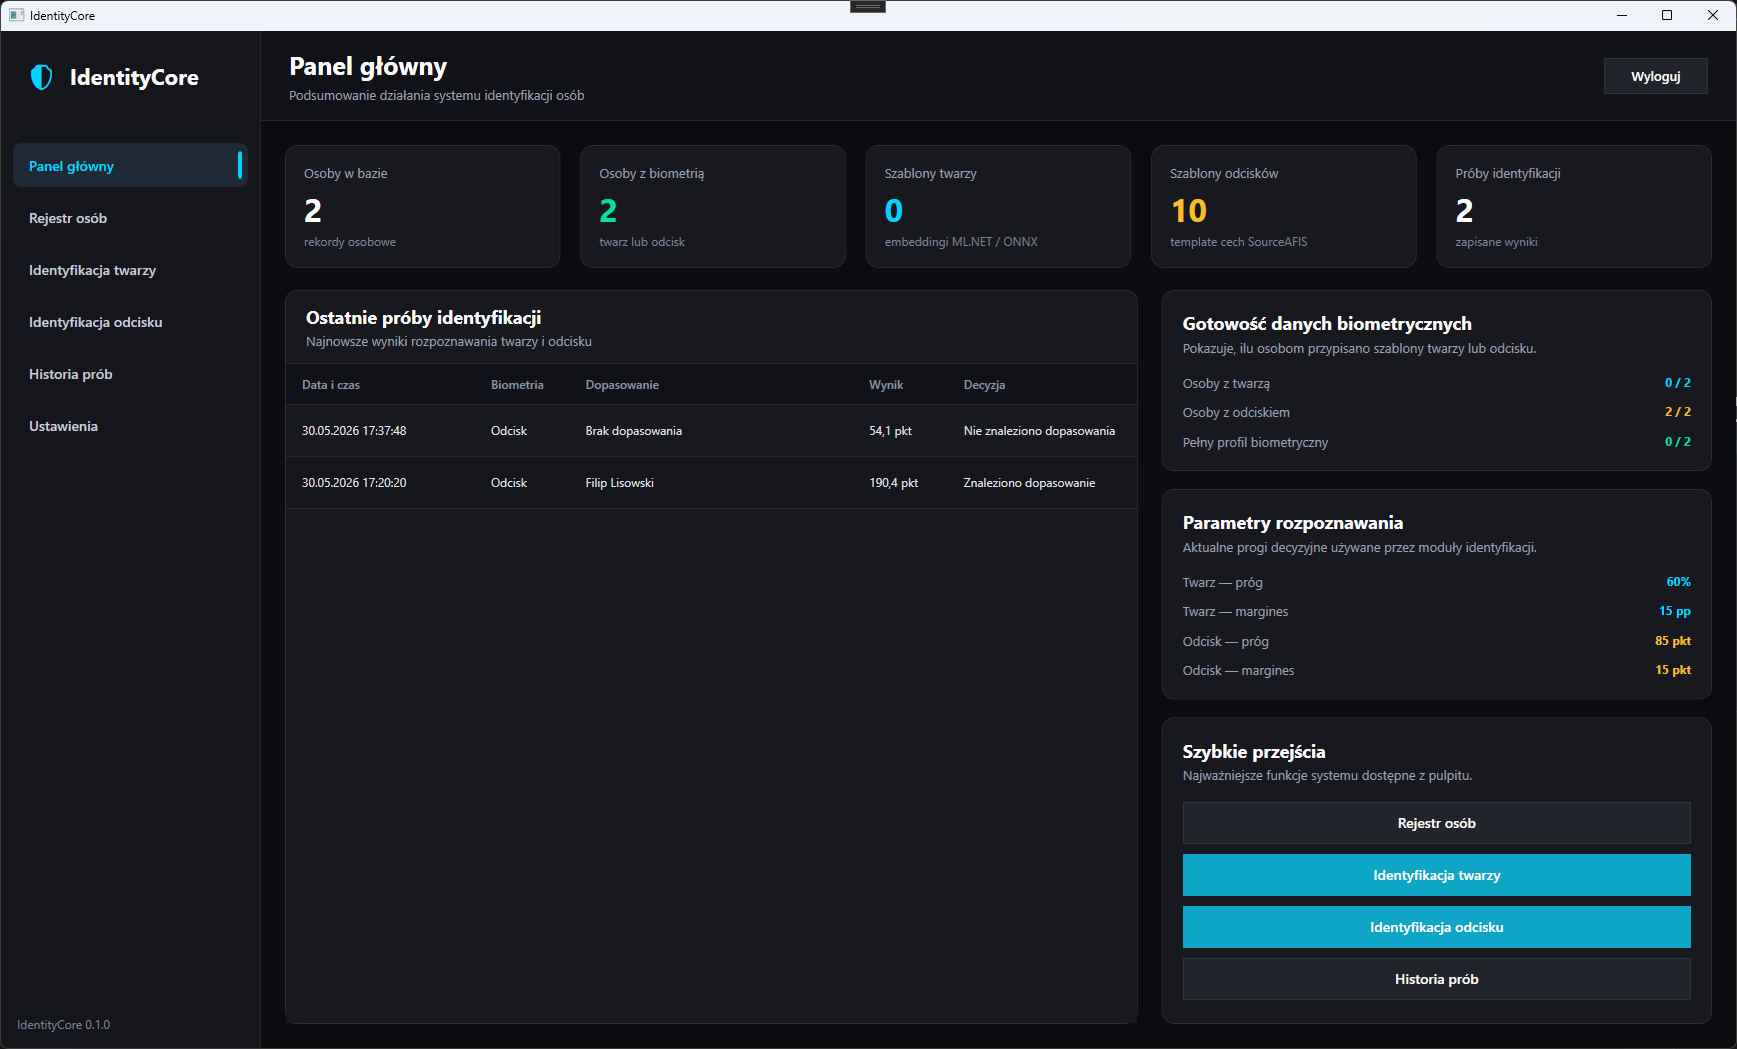
\includegraphics[width=0.98\textwidth]{figures/ui/ui_02_dashboard.png}
    \caption{Panel główny aplikacji po zalogowaniu}
    \label{fig:ui-dashboard}
\end{figure}

\newpage

\section{Rejestr osób i profil osoby}

Widok rejestru osób łączy listę osób zapisanych w systemie z panelem szczegółów aktualnie wybranego profilu. W górnej części widoku znajdują się kafle podsumowujące liczbę osób w bazie, liczbę osób z przypisanymi danymi biometrycznymi oraz liczbę próbek twarzy i odcisków. Poniżej, po lewej stronie, znajduje się tabela osób zawierająca identyfikator osoby, imię i nazwisko, dział lub jednostkę oraz datę dodania. Z poziomu tabeli operator może otworzyć wybrany profil.

\bigskip

Prawa część widoku przedstawia panel profilu osoby. Zawiera zdjęcie profilowe, podstawowe dane osoby, informacje o próbkach twarzy i odcisku palca oraz przyciski umożliwiające rejestrację danych biometrycznych. W tym samym obszarze znajdują się pola edycji danych osobowych oraz przyciski \texttt{Zapisz zmiany} i \texttt{Usuń osobę}. Dzięki temu widok rejestru pełni jednocześnie funkcję listy osób, panelu szczegółów oraz miejsca zarządzania podstawowymi danymi osoby i jej materiałem biometrycznym.

\bigskip

\begin{figure}[H]
    \centering
    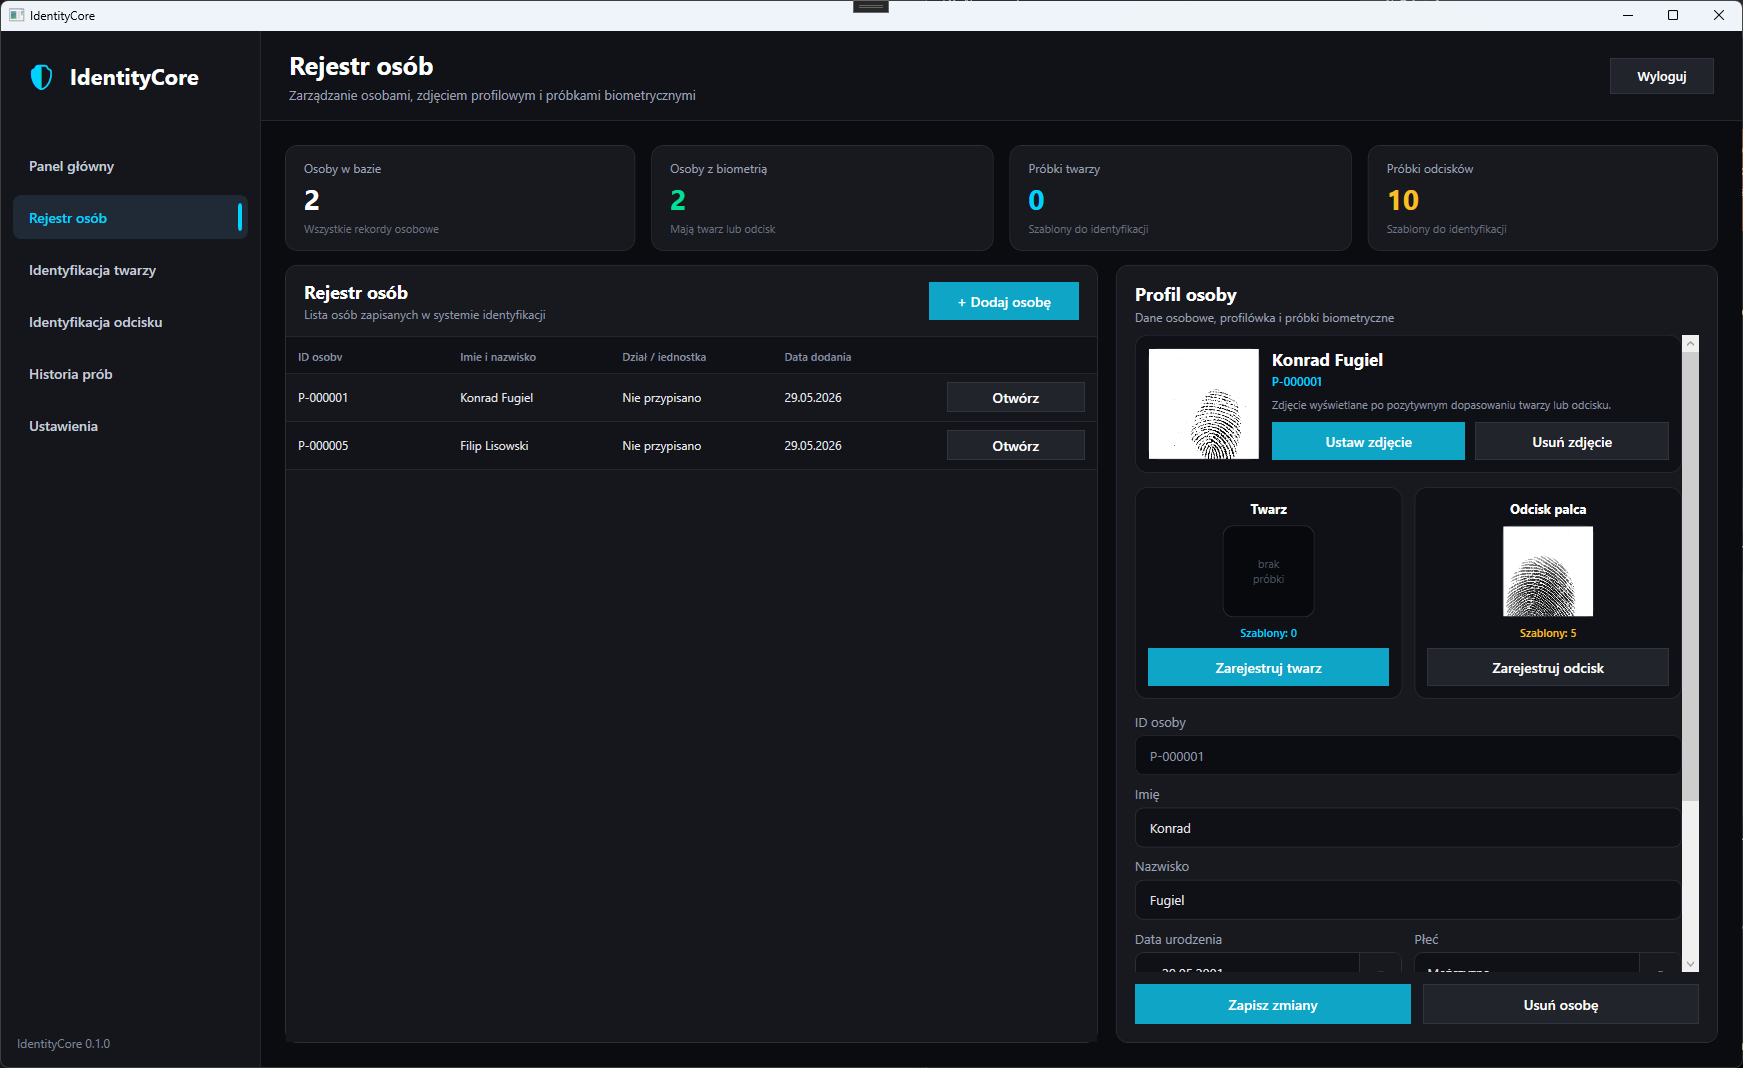
\includegraphics[width=0.98\textwidth]{figures/ui/ui_03_person_registry.png}
    \caption{Rejestr osób wraz z panelem profilu wybranej osoby}
    \label{fig:ui-person-registry}
\end{figure}

\newpage

\section{Widok identyfikacji twarzy}

Widok identyfikacji twarzy został podzielony na trzy główne obszary: źródło biometryczne, analizę biometryczną oraz wynik identyfikacji. Po lewej stronie znajduje się panel z podglądem obrazu oraz przyciskami \texttt{Uruchom kamerę}, \texttt{Wyłącz kamerę}, \texttt{Zrób zdjęcie} i \texttt{Wczytaj obraz}. Oznacza to, że operator może skorzystać zarówno z kamery, jak i z wcześniej przygotowanego pliku graficznego. Widok jasno informuje, że obsługiwane źródła to kamera internetowa oraz pliki obrazów.

\bigskip

Środkowa część widoku prezentuje przebieg analizy. Pokazane są informacje o modelu, jakości próbki, źródle danych oraz bazie wzorców. Poniżej znajduje się lista etapów, takich jak detekcja twarzy, normalizacja obrazu, ekstrakcja cech, porównanie z bazą oraz decyzja systemu. Na dole widoczny jest pasek postępu i przycisk uruchamiający identyfikację. Prawy panel służy do prezentacji wyniku: pokazuje najlepsze dopasowanie, dane osoby, wynik podobieństwa, decyzję systemu oraz listę najbliższych dopasowań. W stanie początkowym aplikacja informuje, że analiza nie została jeszcze wykonana.

\bigskip

\begin{figure}[H]
    \centering
    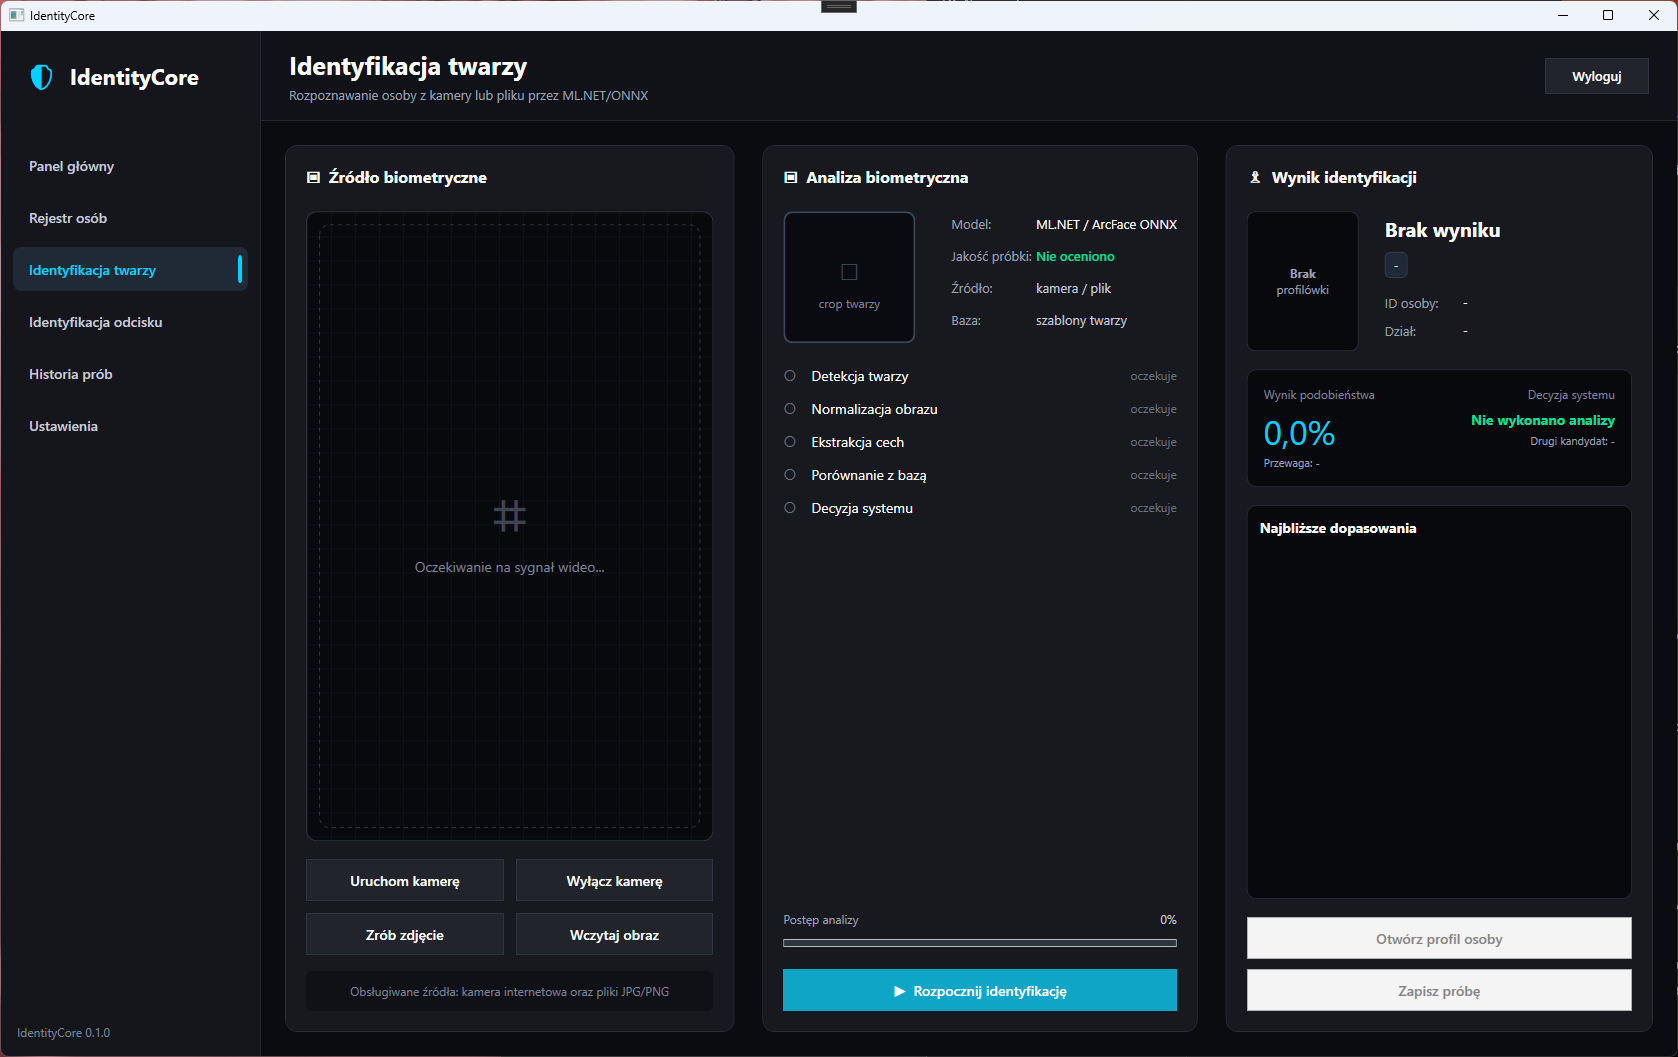
\includegraphics[width=0.98\textwidth]{figures/ui/ui_04_face_identification_input.png}
    \caption{Widok identyfikacji twarzy przed uruchomieniem analizy}
    \label{fig:ui-face-identification}
\end{figure}

\newpage

\section{Widok identyfikacji odcisku palca}

Widok identyfikacji odcisku palca ma podobny układ do modułu twarzy, ale jest dostosowany do pracy z obrazem odcisku. Lewy panel odpowiada za źródło biometryczne i umożliwia wczytanie obrazu odcisku palca z pliku. Widoczny jest duży obszar przeznaczony na podgląd próbki oraz przycisk \texttt{Wczytaj obraz odcisku}. Pod panelem znajduje się informacja o obsługiwanych formatach obrazów oraz o tym, że próbki mogą pochodzić z aplikacji skanera.

\bigskip

Środkowa część widoku pokazuje analizę odcisku palca. Operator widzi informacje o szablonie, cechach, progu oraz kontroli, a także kolejne etapy analizy: wczytanie obrazu, utworzenie template cech, porównanie template z bazą, ocenę wyniku dopasowania i decyzję systemu. Na dole znajduje się pasek postępu oraz przycisk rozpoczęcia analizy. Prawy panel prezentuje najlepsze dopasowanie, identyfikator osoby, dział, wynik punktowy oraz decyzję. W stanie początkowym widok pokazuje brak wyniku i informację, że analiza nie została jeszcze wykonana.

\bigskip

\begin{figure}[H]
    \centering
    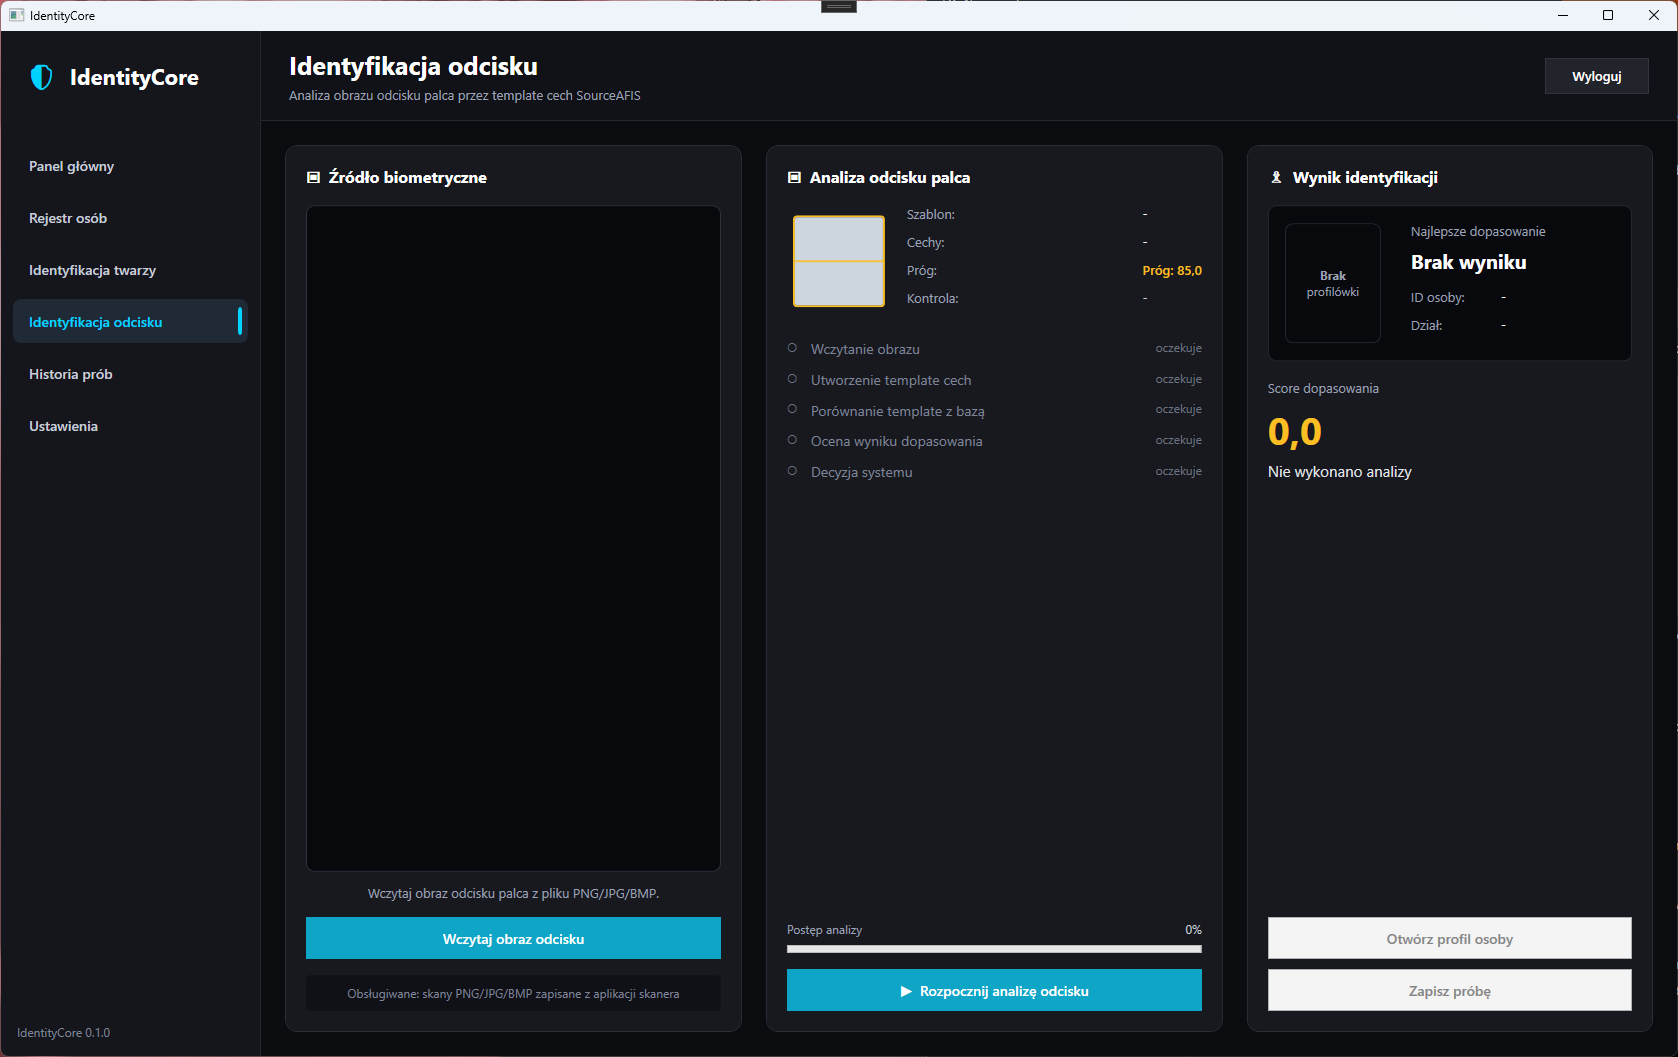
\includegraphics[width=0.98\textwidth]{figures/ui/ui_05_fingerprint_identification_input.png}
    \caption{Widok identyfikacji odcisku palca przed uruchomieniem analizy}
    \label{fig:ui-fingerprint-identification}
\end{figure}

\newpage

\section{Historia prób identyfikacji}

Widok historii prób identyfikacji służy do przeglądania zapisanych zdarzeń związanych z analizą twarzy i odcisku palca. W górnej części ekranu znajdują się liczniki przedstawiające łączną liczbę prób, liczbę znalezionych dopasowań oraz liczbę prób bez dopasowania. Niżej umieszczono tabelę historii, w której widoczne są takie informacje jak data i czas próby, typ biometrii, dopasowanie, wynik, decyzja oraz plik wejściowy. Nad tabelą znajdują się filtry oraz przycisk odświeżania danych.

\bigskip

Po prawej stronie widoku znajduje się panel szczegółów wybranej próby. Pokazuje on wynik, datę próby, typ biometrii, najlepsze dopasowanie oraz plik wejściowy. Taki układ pozwala operatorowi najpierw przeglądać zbiorczą listę prób, a następnie odczytać szczegóły konkretnego zdarzenia bez przechodzenia do innego modułu. Widok historii nie służy w tym rozdziale do oceny skuteczności systemu, ale pokazuje, w jaki sposób aplikacja prezentuje zapisane wyniki pracy modułów identyfikacji.

\bigskip

\begin{figure}[H]
    \centering
    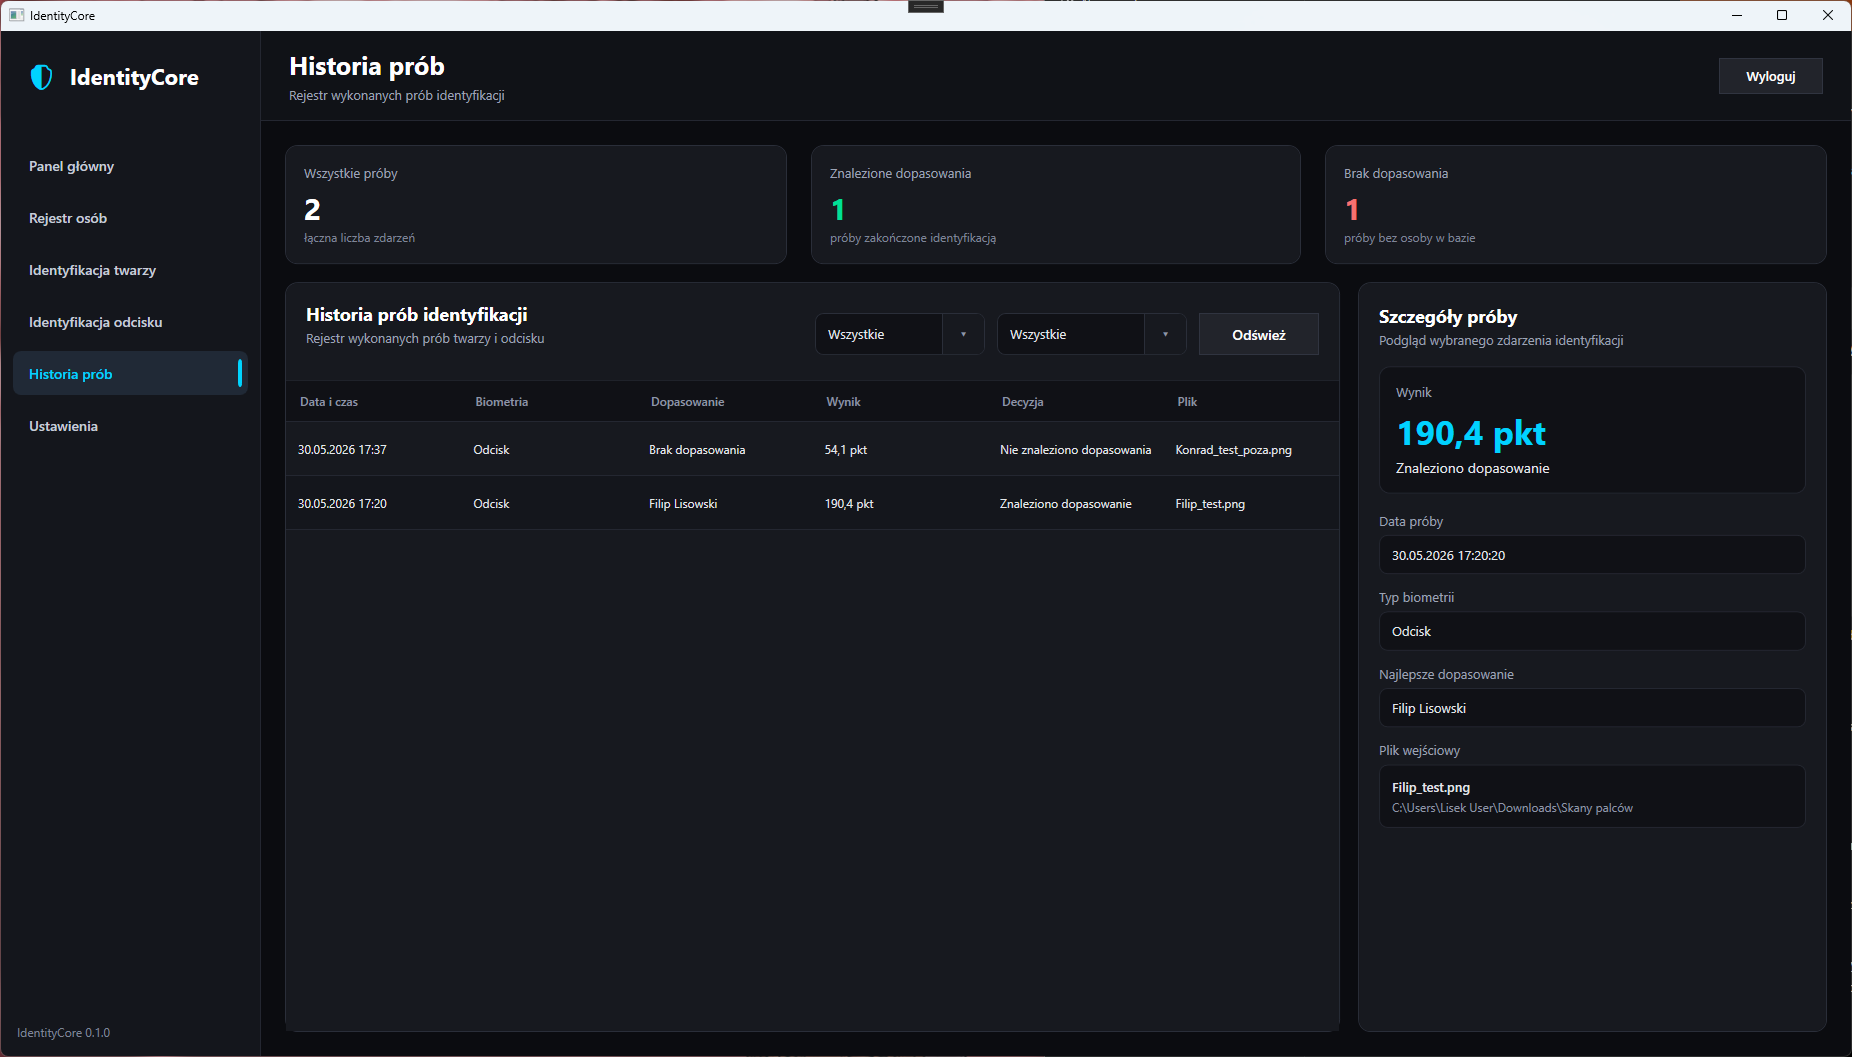
\includegraphics[width=0.98\textwidth]{figures/ui/ui_09_history.png}
    \caption{Widok historii prób identyfikacji}
    \label{fig:ui-history}
\end{figure}

\newpage

\section{Ustawienia systemu}

Widok ustawień prezentuje parametry decyzyjne oraz informacje o modułach biometrycznych. W górnej części ekranu znajdują się kafle opisujące moduł twarzy, moduł odcisku palca oraz sposób prezentacji decyzji systemu. W głównej części widoku umieszczono suwaki i pola wartości dla progów oraz marginesów: minimalnego wyniku podobieństwa twarzy, minimalnej przewagi nad drugim kandydatem, minimalnego wyniku SourceAFIS oraz minimalnej przewagi dla odcisku palca.

\bigskip

Prawa część widoku zawiera informacje o ustawieniach systemu, wykorzystywanych modułach oraz zasobach lokalnych. Widoczne są między innymi odniesienia do modelu \texttt{MLModels/arcface.onnx} oraz katalogów używanych przez aplikację. Na dole panelu znajdują się przyciski \texttt{Zapisz progi} i \texttt{Domyślne}. Pierwszy służy do zapisania aktualnie ustawionych wartości, a drugi do przywrócenia parametrów domyślnych. W tym rozdziale ustawienia są opisane wyłącznie jako element interfejsu, bez analizowania ich wpływu na wyniki identyfikacji.

\bigskip

\begin{figure}[H]
    \centering
    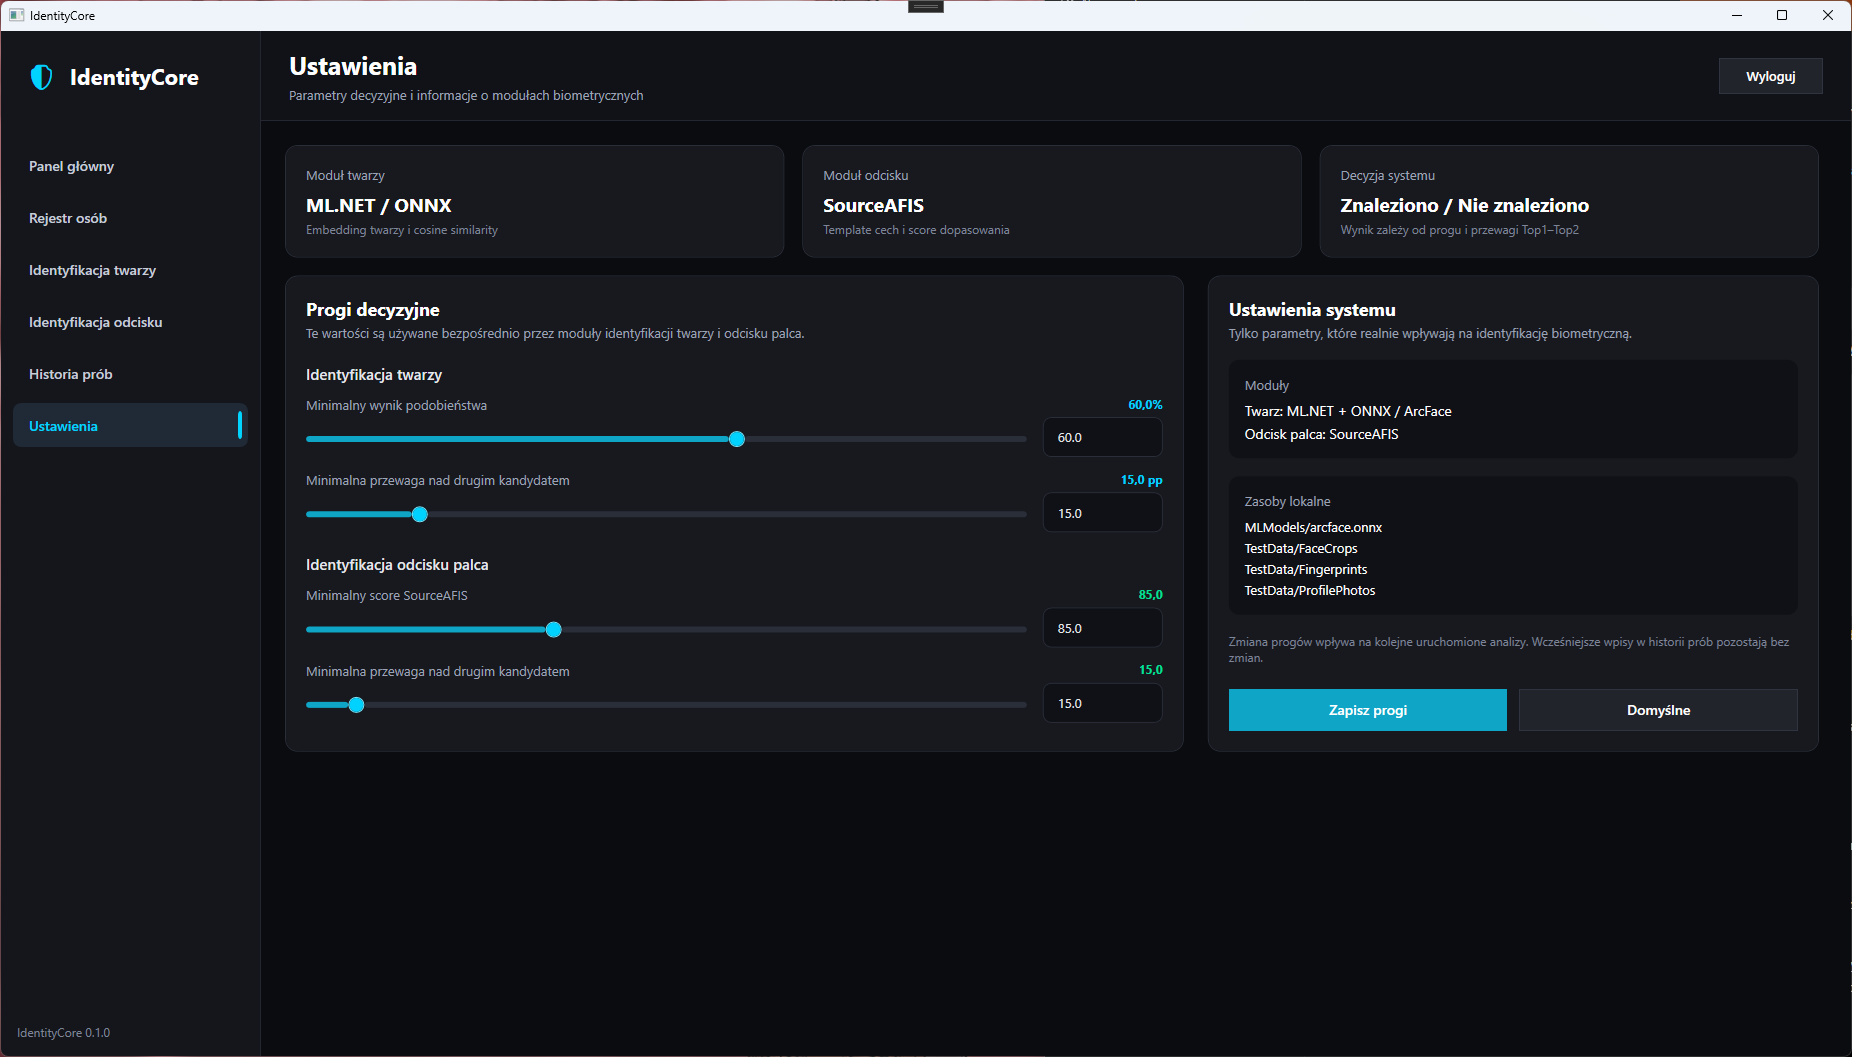
\includegraphics[width=0.98\textwidth]{figures/ui/ui_10_settings.png}
    \caption{Widok ustawień parametrów systemu}
    \label{fig:ui-settings}
\end{figure}

\section{Komunikaty i informacje zwrotne dla operatora}

Aplikacja przekazuje operatorowi informacje zwrotne bez konieczności otwierania osobnych okien dla każdego etapu pracy. W widokach identyfikacji widoczne są statusy etapów analizy, paski postępu, informacje o oczekiwaniu na wykonanie operacji oraz komunikaty o braku wyniku. Operator może więc kontrolować, czy dane wejściowe zostały wczytane, czy analiza została uruchomiona i czy system zakończył proces decyzją.

Wyniki pracy systemu są prezentowane w wydzielonych panelach. W zależności od modułu operator widzi najlepsze dopasowanie, identyfikator osoby, dział, wynik podobieństwa lub punktację, decyzję systemu oraz możliwość otwarcia profilu osoby lub zapisania próby. Historia prób pozwala natomiast wrócić do wcześniejszych zdarzeń i sprawdzić ich szczegóły. Wspólną cechą interfejsu jest wyraźne oddzielenie danych wejściowych, przebiegu analizy i rezultatu, co porządkuje sposób korzystania z aplikacji.